%% osm-applications.tex
%%


\section{Applications}

\frame[plain]{  \heading{Plan de la Présentation}
\ecmsetupplan
\begin{itemize}
  \item[\small $\Diamond$] Introduction
  \item[\small $\Diamond$] Fonctionnement
  \item[\small $\Diamond$] {\color{purple}\textbf{Applications}}
  \item[\small $\Diamond$] Conclusions
\end{itemize}
}



%% http://www.foss4g2007.org/presentations/view.php?abstract_id=56


\frame { \heading{Utilisations des données} \vfil

  %% http://wiki.openstreetmap.org/index.php/Fr:Using_OpenStreetMap
  
  %% http://fredericbonifas.free.fr/osm.html

  %% http://wiki.navit-project.org/images/thumb/f/fa/FBZH-gtk.png/800px-FBZH-gtk.png
  
  \begin{minipage}{0.8\textwidth}
  \begin{itemize}
  \item guidage temps réel (applications: pyroute, navit, GPSDrive,
    gosmore, roadnav) 
  \item cartes et applications de routage thématiques
    \begin{itemize}
    \item spécifique vélo ou piéton ou bâteau
    \item carte des châteaux d'une zone viticole
    \item préparation d'un \textit{pub crawl}
    \end{itemize}
  \item utiliser les données dans des simulateurs
    \begin{itemize}
    \item existe pour FlightGear (avec terragear)
    \item idée Guilhem: simulateur de conduite automobile
    \end{itemize}
  \item permet un réalisme troublant
    \begin{itemize}
    \item localisations des boîtes aux lettres, points de recyclage,
      toilettes, bornes SOS
    \end{itemize}
  \item insérer votre idée ici: les données sont libres!
  \end{itemize}
  \end{minipage} %
  \begin{minipage}{0.19\textwidth}
    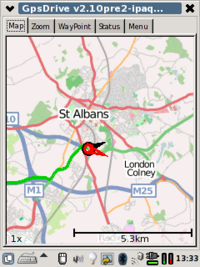
\includegraphics[width=1.5cm]{figures/200px-Gpsdrive_ipaq_screenshot-map-z11}
    \vskip 1cm

    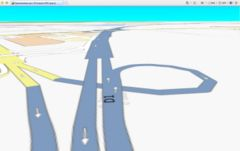
\includegraphics[width=1.5cm]{figures/240px-Now_turn_right2}
    \vskip 1cm
    
    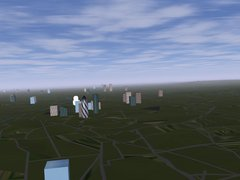
\includegraphics[width=1.5cm]{figures/240px-Osmroads1}
    \vskip 1cm
  \end{minipage}
}

\frame{ \heading{Utilisation sur terminal mobile} \vfil
  \begin{tikzpicture}[remember picture,overlay,font={\footnotesize},text
    width=2cm,text centered]
   \node[xshift=1cm,yshift=-4cm] at (current page.north west) {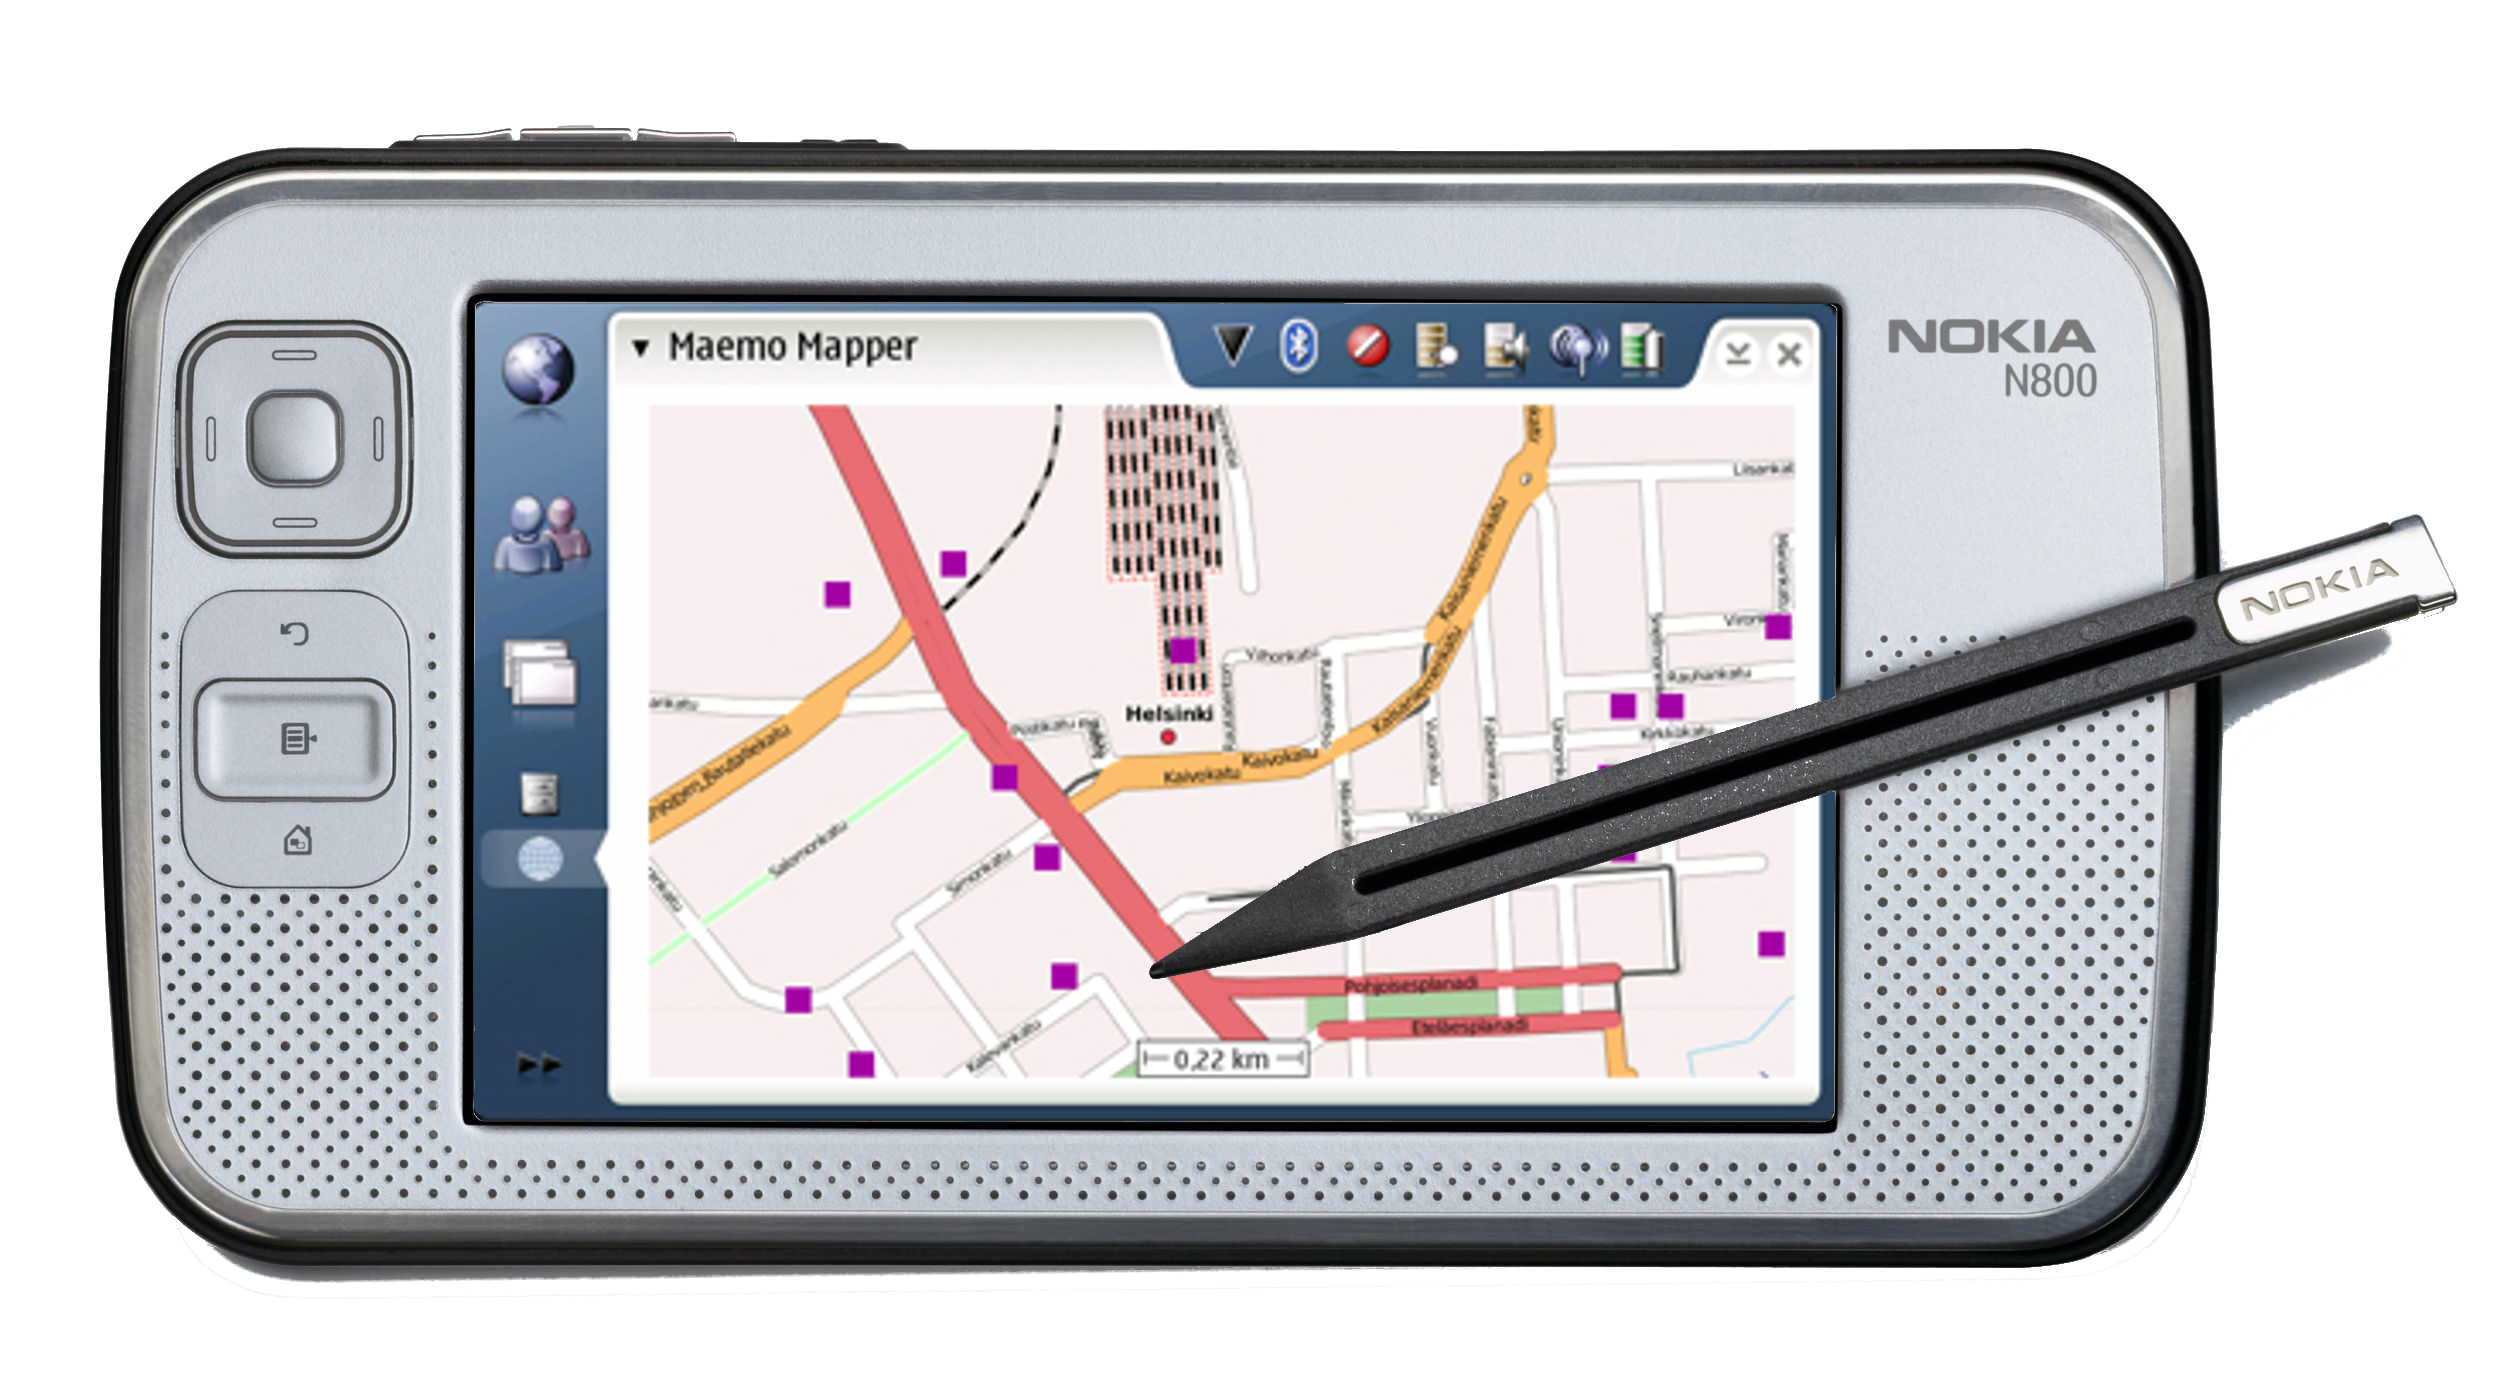
\includegraphics[width=7cm]{figures/osm-N800}};
   \node[xshift=-1cm,yshift=-3cm] at (current page.north east) {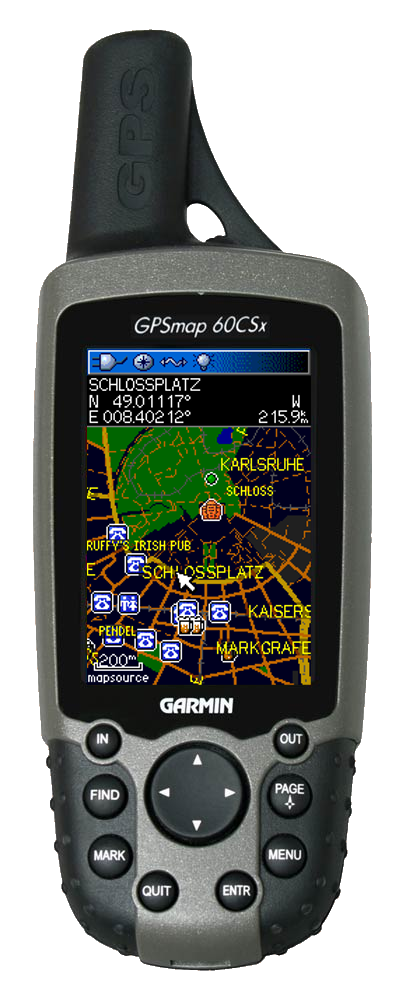
\includegraphics[height=5cm]{figures/OSM-garmin}};
   \node[xshift=-4.7cm,yshift=3.5cm] at (current page.south east) {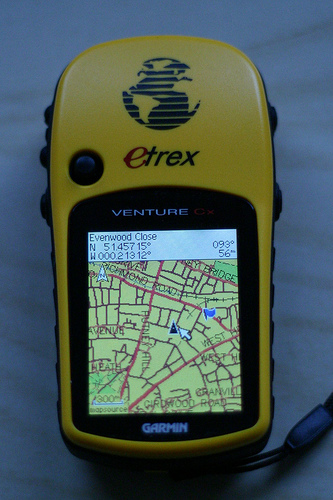
\includegraphics[height=5cm]{figures/OSM-garmin-etrex}};
\end{tikzpicture}
}


%% http://www.geographie.uni-bonn.de/karto/osm-3d/screenshots.en.htm

%% EOF
